\section{78 - MAT - AG 2.4, AN 4.2, AN 4.3, FA 1.4, FA 1.7, FA 3.2, FA 4.1, FA 5.6, WS 1.1, WS 1.2 - Einkommensverteilung - BIFIE Aufgabensammlung}

\begin{langesbeispiel} \item[0] %PUNKTE DES BEISPIELS
	
Der Statistiker Max Lorenz beschrieb bereits im Jahr 1905 statistische Verteilungen mithilfe der nach ihm benannten Lorenz-Kurve. Eine Lorenz-Kurve $f$ kann z.B. zur Beschreibung er Einkommensverteilung in einem Staat herangezogen werden. Je ausgeprägter ihr "`Bauch"' ist, desto größer ist der Einkommensunterschied zwischen niedrigem und hohem Einkommen.

Die Lorenz-Kurve der Einkommensverteilung eines Staates, in dem alle Personen bis auf eine Person nichts verdienen und diese eine Person alles bekommt, wird in der nachstehenden Grafik durch die punktrierten Linien (Katheten eines rechtwinkeligen Dreiecks) dargestellt. Das andere Extrem ist ein Staat, in dem alle Personen gleich viel verdienen. In diesem Fall die die Lorenz-Kurve zu einer Geraden $h$, welche durch die strichlierte Linie dargestellt ist. Zwischen den beiden Extremen verläuft die Lorenz-Kurve $f$ eines Staates.\leer

Jeder Punkt $P=(x|f(x))$ auf der Kurve $f$ steht für folgende Aussage: Die einkommensschwächsten $x$\,\% aller Haushalte beziehen $f(x)$\,\% des Gesamteinkommens."'

\begin{center}
	\resizebox{0.7\linewidth}{!}{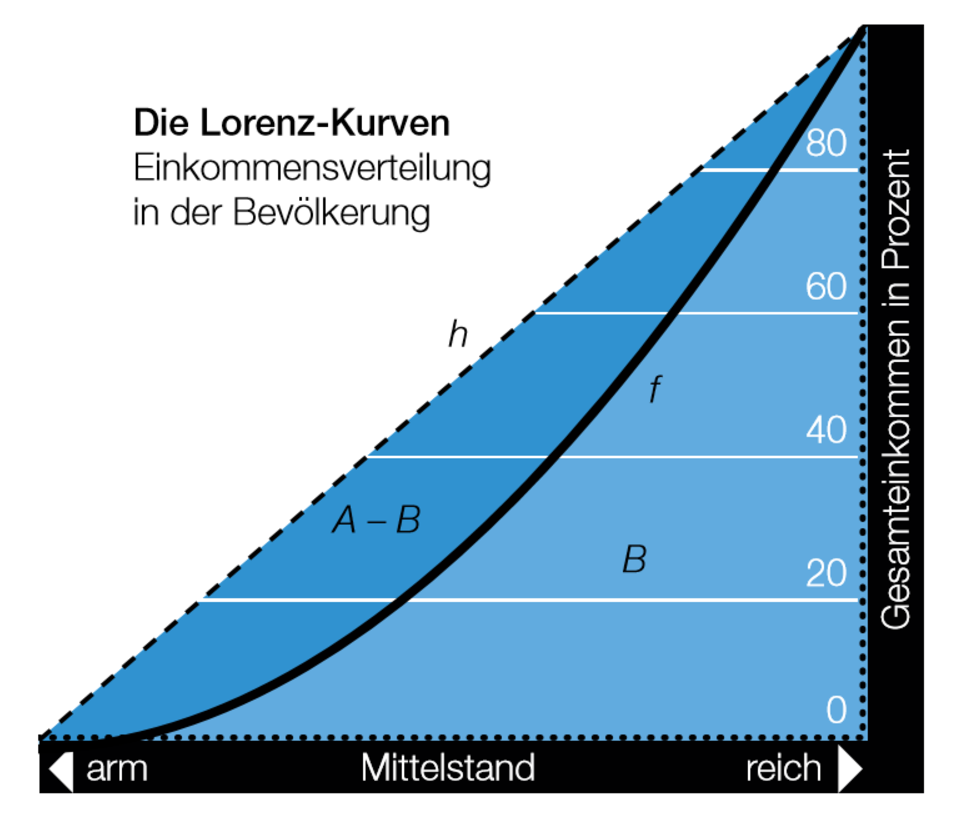
\includegraphics{../Bilder/Bild78-1.eps}}
\end{center}

Der Flächeninhalt des rechtwinkligen Dreiecks wird mit $A$ bezeichnet. Der Graph der Lorenz-Kurve $f$ schließt mit den beiden Katheten des rechtwinkeligen Dreiecks eine Fläche mit Inhalt $B$ ein. Setzt man den Inhalt der Fläche zwischen der Lorenz-Kurve $f$ und der Geraden $h$ mit der Dreiecksfläche $A$ in Bezug, erhält man den Gini-Ungleichheitskoeffizienten $GUK=\frac{A-B}{A}$, eine Zahl zwischen null und ein. Je kleiner der GUK ist, desto gleichmäßiger ist das Gesamteinkommen auf die Bevölkerung verteilt.\leer

In der nachstehenden Grafik ist die Einkommensverteilung in Österreich in Prozent der gesamten Bruttobezüge im jahr 2006 dargestellt. Daraus ist z.B. abzulesen, dass jene 20\,\% der Bevölkerung mit den niedrigsten Bruttoeinkommen nur 2,2\,\% des Gesamtbruttoeinkommens erhalten haben.

\begin{center}
	\resizebox{0.8\linewidth}{!}{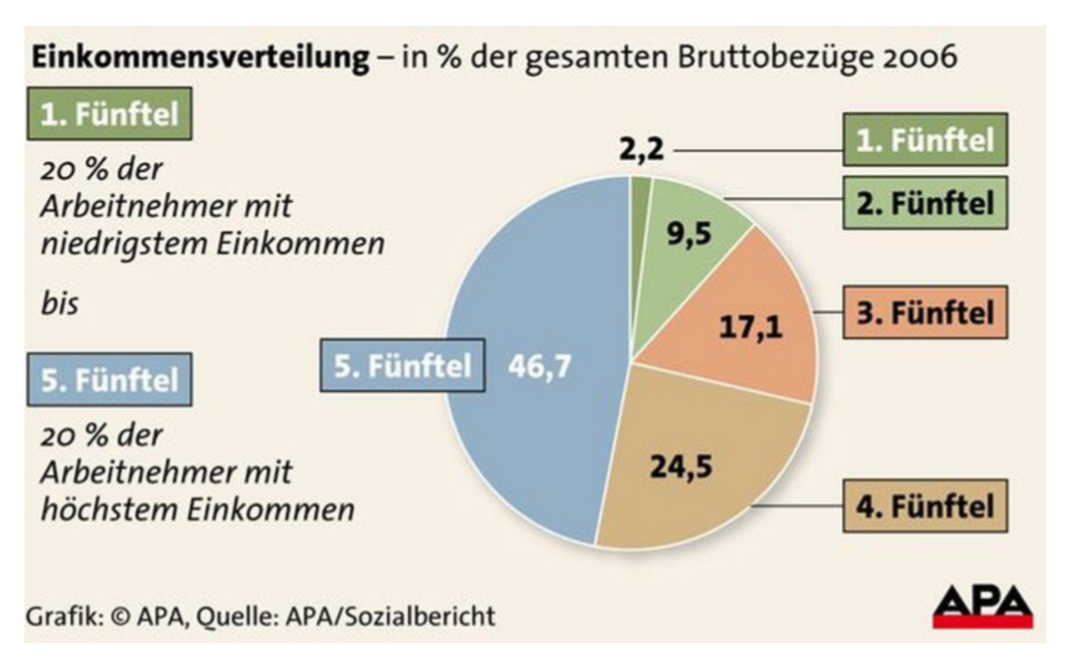
\includegraphics{../Bilder/Bild78-2.eps}}
\end{center}

\begin{scriptsize}\begin{singlespace}Quelle: http://diepresse.com/home/wirtschaft/economist/446997/Sozialbericht\_Einkommen-in-Oesterreich-ungleicher-verteilt [04.05.2017].\end{singlespace}\end{scriptsize}

\subsection{Aufgabenstellung:}
\begin{enumerate}
	\item Zeichne die Lorenzkurve für die Einkommensverteilung der Bruttobezüge in Österreich im Jahr 2006 in den nachstehenden Grafik als Streckenzug ein!
	
	\begin{center}
		\resizebox{0.8\linewidth}{!}{\psset{xunit=8.0cm,yunit=8.0cm,algebraic=true,dimen=middle,dotstyle=o,dotsize=4pt 0,linewidth=0.8pt,arrowsize=3pt 2,arrowinset=0.25}
\begin{pspicture*}(-0.08726875556452825,-0.12333898008375876)(1.1526748130814817,1.0658128492748549)
\multips(0,0)(0,0.1){12}{\psline[linestyle=dashed,linecap=1,dash=1.5pt 1.5pt,linewidth=0.4pt,linecolor=lightgray]{c-c}(0,0)(1.1526748130814817,0)}
\multips(0,0)(0.2,0){7}{\psline[linestyle=dashed,linecap=1,dash=1.5pt 1.5pt,linewidth=0.4pt,linecolor=lightgray]{c-c}(0,0)(0,1.0658128492748549)}
\psaxes[labelFontSize=\scriptstyle,xAxis=true,yAxis=true,Dx=0.2,Dy=0.1,ticksize=-2pt 0,subticks=2]{->}(0,0)(0.,0.)(1.1526748130814817,1.0658128492748549)
\begin{scriptsize}
\rput[tl](0.023837298973644686,1.0368091461197668){Einkommensanteil (relativ)}
\rput[tl](0.5727012083922189,0.05068323884677006){Einkommensgruppe (Anteil relativ)}
\psline[linewidth=1.2pt,linestyle=dashed,dash=1pt 1pt](0.,0.)(1.,1.)
\rput[tl](0.5660348451199285,0.6275346682646341){h}
\psline[linewidth=1.2pt]{->}(0.7,-0.09)(0.89,-0.09)
\psline[linewidth=1.2pt]{->}(0.49,-0.09)(0.3,-0.09)
\rput[tl](0.49937121239702476,-0.07983342535112656){Mittelstand}
\rput[tl](0.92,-0.075){reich}
\rput[tl](0.2,-0.07983342535112656){arm}
\end{scriptsize}
\end{pspicture*}}
	\end{center}
	
	Berechne mithilfe des eingezeichneten Streckenzuges den GUK für die Bruttobezüge in Österreich für das Jahr 2006!\leer
	
	\item Die Verteilung der Bruttoeinkommen in Österreich im Jahr 2006 soll durch eine Polynomfunktion $p$ so modelliert werden, dass alle Daten, die aus dem Kreisdiagramm aus der Einleitung abgelesen werden können mit Funktionswerten dieser Polynomfunktion übereinstimmen.\leer
	
	Begründe, welchen Grad die Polynomfunktion $p$ bei konkreter Berechnung (maximal) hat!\leer
	
	Begründe, warum eine Exponentialfunktion $e$ mit $e(x)=a\cdot b^x (a,b\in\mathbb{R}^+$ nicht für die Modellierung einer Lorenz-Kurve geeignet ist!\leer
	
	\item Um politische Maßnahmen abschätzen zu können, werden verschiedene Szenarien entworfen. So soll beispielsweise für die Bruttoeinkommen langfristig eine Lorenz-Kurve angestrebt werden, die durch die Funktion $g$ mit der Funktionsgleichung $g(x)=0,245\cdot x³+0,6\cdot x²+0,155\cdot x$ beschrieben werden kann.\leer
	
	Gib eine Gleichung an, mit der der GUK für die angestrebte Einkommensverteilung berechnet werden kann, und ermittle diesen GUK!\leer
	
	Gib mithilfe konkreter Zahlenwerte an, wie sich in diesem Fall die Einkommensverteilung der "`20\,\% der Arbeitnehmer/innen mit den niedrigsten Bruttoeinkommen"' und die Einkommensverteilung der "`20\,\% der Arbeitnehmer/innen mit den höchsten Bruttoeinkommen"' im Vergleich zu den Bruttobezügen im Jahr 2006 in Österreich ändern würde!\leer
	
	\item Für das Jahr 2007 kann die Einkommensverteilung für Österreich mit einem GUK von $0,26$ beschrieben werden.
	
	\begin{scriptsize}\begin{singlespace}Datenquelle: https://de.wikipedia.org/wiki/Liste\_der\_L\%C3\%A4nder\_nach\_Einkommensverteilung [04.05.2017]. \end{singlespace}\end{scriptsize}\leer
	
	Angenommen, die Lorenz-Kurve für die Einkommenverteilung kann für ein bestimmtes Land, das eine ausgeglichenere Einkommensverteilung als Österreich aufweisen soll, durch eine Potenzfunktion $h$ mit $h(x)=a\cdot x^z+b$ mit $a,b,z\in\mathbb{R}$ beschrieben werden.\leer
	
	Gib an, welche Werte die Parameter $a$ und $b$ haben müssen, und begründe deine Wahl!\leer
	
	Gib eine Ungleichung an, die für das Jahr 2007 einen Zusammenhang zwischen dem GUK von Österreich und dem GUK von demjenigen Land, das eine ausgeglichenere Einkommensverteilung als Österreich aufweisen soll, beschreibt! Ermittle für diesen Fall einen möglichen Wert für den Exponenten $z$ mit $z>1$!
	
\end{enumerate}

\antwort{
\begin{enumerate}
	\item \subsection{Lösungserwartung:} 

\begin{center}
		\resizebox{0.8\linewidth}{!}{\psset{xunit=8.0cm,yunit=8.0cm,algebraic=true,dimen=middle,dotstyle=o,dotsize=4pt 0,linewidth=0.8pt,arrowsize=3pt 2,arrowinset=0.25}
\begin{pspicture*}(-0.08726875556452825,-0.12333898008375876)(1.1526748130814817,1.0658128492748549)
\multips(0,0)(0,0.1){12}{\psline[linestyle=dashed,linecap=1,dash=1.5pt 1.5pt,linewidth=0.4pt,linecolor=lightgray]{c-c}(0,0)(1.1526748130814817,0)}
\multips(0,0)(0.2,0){7}{\psline[linestyle=dashed,linecap=1,dash=1.5pt 1.5pt,linewidth=0.4pt,linecolor=lightgray]{c-c}(0,0)(0,1.0658128492748549)}
\psaxes[labelFontSize=\scriptstyle,xAxis=true,yAxis=true,Dx=0.2,Dy=0.1,ticksize=-2pt 0,subticks=2]{->}(0,0)(0.,0.)(1.1526748130814817,1.0658128492748549)
\begin{scriptsize}
\rput[tl](0.023837298973644686,1.0368091461197668){Einkommensanteil (relativ)}
\rput[tl](0.5727012083922189,0.05068323884677006){Einkommensgruppe (Anteil relativ)}
\psline[linewidth=1.2pt,linestyle=dashed,dash=1pt 1pt](0.,0.)(1.,1.)
\rput[tl](0.5660348451199285,0.6275346682646341){h}
\psline[linewidth=1.2pt]{->}(0.7,-0.09)(0.89,-0.09)
\psline[linewidth=1.2pt]{->}(0.49,-0.09)(0.3,-0.09)
\rput[tl](0.49937121239702476,-0.07983342535112656){Mittelstand}
\rput[tl](0.92,-0.075){reich}
\rput[tl](0.2,-0.07983342535112656){arm}
\psline[linewidth=1.2pt](0.,0.)(0.2,0.022)
\psline[linewidth=1.2pt](0.2,0.022)(0.4,0.117)
\psline[linewidth=1.2pt](0.4,0.117)(0.6,0.288)
\psline[linewidth=1.2pt](0.6,0.288)(0.8,0.533)
\psline[linewidth=1.2pt](0.8,0.533)(1.,1.)
\rput[tl](0.5060375756693152,0.18764517041246404){f}
\end{scriptsize}
\end{pspicture*}}
	\end{center}
	
	Der Inhalt der Fläche zwischen dem Polygonzug $f$ und der Strecke $h$ beträgt 0,208 Flächeneinheiten (die Ermittlung des Flächeninhalts zwischen der waagrechten Achse und dem Streckenzug kann z.B. aus zwei Dreiecksflächen und drei Trapezflächen erfolgen).\leer
	
	$\Rightarrow GUK=\frac{0,208}{0,5}=0,416$

	\item \subsection{Lösungserwartung:}
	
	Aus den Daten des Kreisdiagramms ergeben sich (für die Argumente $x=0, x=0,2, x=0,4, x=0,6, x=0,8, x=1$) sechs Funktionswerte von $p$ und somit sechs "`Bedingungen"' für die Koeffizienten der Funktionsgleichung. Eine Polynomfunktion fünften Grades hat sechs Koeffizienten und ist daher geeignet.
	
	\textit{(Anmerkung: Bei "`besonderer"' Lage der Punkte kann auch ein Grad kleiner als fünf ausreichend sein.}\leer
	
	Jede Lorenz-Kurve verläuft durch den Punkt $(0|0)$. Da eine Exponentialfunktion $e$ mit $e(x)=a\cdot b^x$ $(a,b\in\mathbb{R}^+)$ nicht durch den Koordinatenursprung verläuft, ist sie nicht für die Modellierung geeignet.

\item \subsection{Lösungserwartung:}
	
$GUK=\dfrac{0,5-\int^1_0{(0,245x³+0,6x²+0,155x)dx}}{0,5}=0,3225$\leer

$g(0,2)\approx 0,057$

$g(0,8)\approx 0,633$\leer

Der Einkommensanteil der "`20\,\% mit den niedrigsten Bruttoeinkommen"' würde (um ca. 3,5 Prozentpunkte) von 2,2\,\% auf ca. 5,7\,\% steigen.\leer

Der Einkommensanteil der "`20\,\% mit den höchsten Bruttoeinkommen"' würde (um ca. 10 Prozentpunkte) von 46,7\,\% auf 36,7\,\% sinken.
\item \subsection{Lösungserwartung:}
	
$b=0$, da der Graph durch den Punkt $(0|0)$ verlaufen muss

$a=1$, da der Graph durch den Punkt $(1|1)$ verlaufen muss

$$\frac{0,5-\int^1_0{x^z}dx}{0,5}<0,26$$

$z\in\left(1;\frac{63}{37}\right)$

\end{enumerate}}
		\end{langesbeispiel}